%%%%%%%%%%%%%%%%%%%%%%%%%%%%%%%%%%%%%%%%%%%%%%%%%%%%%%%%%%%%%%%%%%%%
%% I, the copyright holder of this work, release this work into the
%% public domain. This applies worldwide. In some countries this may
%% not be legally possible; if so: I grant anyone the right to use
%% this work for any purpose, without any conditions, unless such
%% conditions are required by law.
%%%%%%%%%%%%%%%%%%%%%%%%%%%%%%%%%%%%%%%%%%%%%%%%%%%%%%%%%%%%%%%%%%%%

\documentclass{beamer}
\usetheme[faculty=phil]{fibeamer}
\usepackage[utf8]{inputenc}
\usepackage[
  main=english
]{babel}
%% These macros specify information about the presentation
\title{Classical Black Holes} %% that will be typeset on the
\subtitle{07. Geodesics around a Rotating Black Hole} %% title page.
\author{Edward Larra\~{n}aga}
%% These additional packages are used within the document:
\usepackage{ragged2e}  % `\justifying` text
\usepackage{booktabs}  % Tables
\usepackage{tabularx}
\usepackage{tikz}      % Diagrams
\usetikzlibrary{calc, shapes, backgrounds}
\usepackage{amsmath, amssymb}
\usepackage{url}       % `\url`s
\usepackage{listings}  % Code listings
\usepackage{siunitx}
\frenchspacing
\begin{document}
\frame{\maketitle}

\AtBeginSection[]{% Print an outline at the beginning of sections
\begin{frame}<beamer>
\frametitle{Outline for Part \thesection}
\tableofcontents[currentsection]
\end{frame}}

\section{Particle Motion around a Black Hole}
\begin{frame}
\Huge
Particle Motion around a Black Hole
\end{frame}

\subsection{Lagrangian Formulation}
\begin{frame}
	\huge
    Lagrangian Formulation
\end{frame}

\begin{frame}{Lagrangian Formulation}
	Stationary and axis-symmetric spacetime
	$$ ds^2 = g_{tt} dt^2 + 2g_{t \varphi} dt d\varphi + g_{rr} dr^2 + g_{\theta \theta} d\theta^2 + g_{\varphi \varphi} d\varphi^2 $$
	\pause
	Lagrangian for a particle moving in a spacetime defined by the metric $g_{\mu\nu}$
	$$ \mathcal{L} = \frac{1}{2} g_{\mu\nu} \dot{x}^\mu \dot{x}^\nu $$
	\pause
	$$ \dot{x}^\mu = \frac{dx^\mu}{d\lambda} $$
\end{frame}

\begin{frame}{Lagrangian Formulation}
	$$ \mathcal{L} = \frac{1}{2} g_{\mu\nu} \dot{x}^\mu \dot{x}^\nu = \frac{1}{2}  \left( \frac{ds}{d\lambda} \right)^2 $$
	\pause	
	$$ \mathcal{L} =\frac{1}{2} \left[ g_{tt} \dot{t}^2 + 2g_{t \varphi} \dot{t} \dot{\varphi} + g_{rr} \dot{r}^2 + g_{\theta \theta} \dot{\theta}^2 + g_{\varphi \varphi} \dot{\varphi}^2 \right] = \frac{1}{2} \delta$$
	\pause
	\[	\delta = 
	\begin{cases}
	0   &\textrm{for photons} \\
	-1  &\textrm{for massive particles}
	\end{cases}	
	\]
\end{frame}

\subsection{Conserved Quantities}
\begin{frame}
	\huge
    Conserved Quantities
\end{frame}

\begin{frame}{Conserved Quantities}	
	$$ \mathcal{L} =\frac{1}{2}  \left[ g_{tt} \dot{t}^2 + 2g_{t \varphi} \dot{t} \dot{\varphi} + g_{rr} \dot{r}^2 + g_{\theta \theta} \dot{\theta}^2 + g_{\varphi \varphi} \dot{\varphi}^2 \right] = \frac{1}{2} \delta$$
	\pause
	\begin{align*}
	p_t &= \frac{\partial \mathcal{L}}{\partial \dot{t}} =  \left[ g_{tt} \dot{t} + g_{t \varphi} \dot{\varphi} \right] = - \varepsilon  \\
	p_\varphi &= \frac{\partial \mathcal{L}}{\partial \dot{\varphi}} = \left[ g_{t \varphi} \dot{t} + g_{\varphi \varphi} \dot{\varphi} \right] = \ell_z 
	\end{align*}
\end{frame}

\begin{frame}{Conserved Quantities}
	\begin{align*}
	\varepsilon &= \frac{E}{m_0} = - g_{tt} \dot{t} - g_{t \varphi} \dot{\varphi}    \\
	\ell_z &= \frac{L_z}{m_0} =  g_{t \varphi} \dot{t} + g_{\varphi \varphi} \dot{\varphi}  
	\end{align*}
\end{frame}

\begin{frame}{Conserved Quantities}
	\begin{align*}
	\dot{t} &= \frac{\varepsilon g_{\varphi \varphi} + \ell_z g_{t \varphi}}{g_{t \varphi}^2 - g_{tt} g_{\varphi \varphi}} \\
	\dot{\varphi} &= - \frac{\varepsilon g_{t \varphi} + \ell_z g_{tt}}{g_{t \varphi}^2 - g_{tt} g_{\varphi \varphi}}  
	\end{align*}	
\end{frame}

\subsection{Effective Potential}
\begin{frame}
	\huge
    Effective Potential
\end{frame}

\begin{frame}{Effective Potential}
	$$ \mathcal{L} =\frac{1}{2} \left[ g_{tt} \dot{t}^2 + 2g_{t \varphi} \dot{t} \dot{\varphi} + g_{rr} \dot{r}^2 + g_{\theta \theta} \dot{\theta}^2 + g_{\varphi \varphi} \dot{\varphi}^2 \right] = \frac{1}{2} \delta$$
	\pause
	\[ g_{rr} \dot{r}^2 + g_{\theta \theta} \dot{\theta}^2 = V_{eff} (r, \theta) \]
	\pause
	\[ V_{eff} (r,\theta) = \frac{\varepsilon^2 g_{\varphi \varphi} + 2 \varepsilon \ell_z g_{t\varphi} + \ell_z^2 g_{tt} }{g_{t\varphi}^2-g_{tt} g_{\varphi\varphi}} + \delta \]
\end{frame}


\begin{frame}{Equations of Motion}
	$$\frac{d}{d\lambda} \left( \frac{\partial \mathcal{L}}{\partial \dot{x}^\alpha} \right) = \frac{\partial \mathcal{L}}{\partial x^\alpha} $$ 
	\pause
	$$\frac{d}{d\lambda} \left(  g_{\mu\alpha} \dot{x}^\mu \right) =  \frac{1}{2} \frac{\partial g_{\mu\nu}}{\partial x^\alpha} \dot{x}^\mu \dot{x}^\nu$$ 
	\pause
	$$\frac{d}{d\lambda} \left( g_{\mu\alpha} \dot{x}^\mu \right) =  \frac{1}{2} \frac{\partial g_{\mu\nu}}{\partial x^\alpha} \dot{x}^\mu \dot{x}^\nu$$ 
\end{frame}


\begin{frame}{Radial Equation of Motion}
	$$\frac{d}{d\lambda} \left( g_{\mu\alpha} \dot{x}^\mu \right) =  \frac{1}{2} \frac{\partial g_{\mu\nu}}{\partial x^\alpha} \dot{x}^\mu \dot{x}^\nu$$ 
	\pause
	$$\frac{d}{d\lambda} \left( g_{\mu r} \dot{x}^\mu \right) =  \frac{1}{2} \frac{\partial g_{\mu\nu}}{\partial r} \dot{x}^\mu \dot{x}^\nu$$
	\pause
	$$\frac{d}{d\lambda} \left( g_{rr} \dot{r} \right) =  \frac{1}{2} \left[ \partial_r g_{tt} \dot{t}^2 + 2\partial_r g_{t \varphi} \dot{t} \dot{\varphi} + \partial_r g_{rr} \dot{r}^2 + \partial_r g_{\theta \theta} \dot{\theta}^2 + \partial_r g_{\varphi \varphi} \dot{\varphi}^2 \right]$$
\end{frame}

\subsection{Equatorial Motion}
\begin{frame}
	\huge
    Equatorial Motion
\end{frame}

\begin{frame}{Effective Potential in the Equatorial Plane}
	Considering equatorial motion, $ \theta = \frac{\pi}{2} $, 
	\pause
	\[ g_{rr} \dot{r}^2 = V_{eff} (r) \]
	\pause
	\[ V_{eff} (r) = \frac{\varepsilon^2 g_{\varphi \varphi} + 2 \varepsilon \ell_z g_{t\varphi} + \ell_z^2 g_{tt} }{g_{t\varphi}^2-g_{tt} g_{\varphi\varphi}} + \delta \]
\end{frame}

\begin{frame}{Schwarzschild Effective Potential in the Equatorial Plane}
	Considering massive particles, $\delta = -1$, moving in the equatorial plane, $ \theta = \frac{\pi}{2} $, around Schwarzschild's geometry,
	\pause
	\[ \frac{1}{2} \dot{r}^2 = \frac{\varepsilon^2 -1}{2} - U_{eff} (r) \]
	\pause	
	\[ U_{eff} (r) = -\frac{M}{r} + \frac{\ell_z^2}{2r^2} - \frac{M\ell_z^2}{r^3} \]
\end{frame}

\begin{frame}{Schwarzschild Effective Potential in the Equatorial Plane}	
	\[ U_{eff} (r) = -\frac{M}{r} + \frac{\ell_z^2}{2r^2} - \frac{M\ell_z^2}{r^3} \]
	\pause
	$-\frac{M}{r}$: Newtonian Potential
	\bigskip
	\pause
	
	$\frac{\ell_z^2}{2r^2}$: Centrifugal Potential (repulsive)
	\bigskip
	\pause
	
	$- \frac{M\ell_z^2}{r^3}$: Relativistic Contribution. Responsible for the ISCO
\end{frame}

\begin{frame}{Schwarzschild Effective Potential in the Equatorial Plane}
	\begin{center}
      \begin{figure}
      	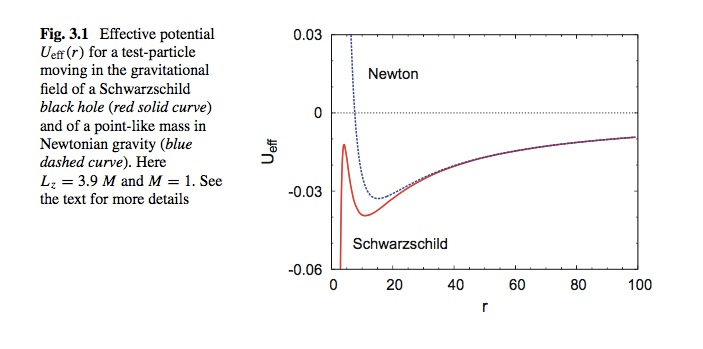
\includegraphics[scale=0.4] {figures/scheffpot.jpeg}
      \end{figure}
	\end{center}	
\end{frame}

\subsection{Equatorial Circular Orbits}
\begin{frame}
	\huge
    Equatorial Circular Orbits
\end{frame}

\begin{frame}{Circular Motion in the Equatorial Plane}
	Circular motion is obtained by the conditions
	\[ \dot{r} = \dot{\theta} = 0 \]
	\pause
	which imply
	\[ \begin{cases}
	 	&V_{eff} = 0\\
	 	&\partial_r V_{eff} = 0
	 	\end{cases} 
	 \]
\end{frame}

\begin{frame}{Equation of a Circular Motion in the Equatorial Plane}
	Another way to calculate the equation of a circular motion in the equatorial plane is taking
	$$\frac{d}{d\lambda} \left( g_{rr} \dot{r} \right) =  \frac{1}{2} \left[ \partial_r g_{tt} \dot{t}^2 + 2\partial_r g_{t \varphi} \dot{t} \dot{\varphi} + \partial_r g_{rr} \dot{r}^2 + \partial_r g_{\theta \theta} \dot{\theta}^2 + \partial_r g_{\varphi \varphi} \dot{\varphi}^2 \right]$$
	\pause
	Considering equatorial motion, $ \theta = \frac{\pi}{2} $, in circular orbits, $\ddot{r} = \dot{r} = \dot{\theta} = 0$, 	
	\pause
	$$\partial_r g_{tt} \dot{t}^2 + 2\partial_r g_{t \varphi} \dot{t} \dot{\varphi} + \partial_r g_{\varphi \varphi} \dot{\varphi}^2 =0$$
\end{frame}

\begin{frame}{Angular Velocity of a Particle in Circular Motion in the Equatorial Plane}
	$$\partial_r g_{tt} \dot{t}^2 + 2\partial_r g_{t \varphi} \dot{t} \dot{\varphi} + \partial_r g_{\varphi \varphi} \dot{\varphi}^2 =0$$
	\pause
	$$ \partial_r g_{\varphi \varphi} \left(\frac{\dot{\varphi}}{\dot{t}}\right)^2 + 2\partial_r g_{t \varphi} \left(\frac{\dot{\varphi}}{\dot{t}}\right) + \partial_r g_{tt}=0$$
	\pause
	$$\Omega =\frac{\dot{\varphi}}{\dot{t}} = \frac{-\partial_r g_{t \varphi} \pm \sqrt{\left(\partial_r g_{t \varphi}\right)^2 - \left(\partial_r g_{tt} \right) \left( \partial_r g_{\varphi \varphi}\right) ) }}{\partial_r g_{\varphi \varphi}} $$	
\end{frame}

\begin{frame}{Conserved Quantities for a Particle in Circular Motion}
	\[ \mathcal{L} =\frac{1}{2} \left[ g_{tt} \dot{t}^2 + 2g_{t \varphi} \dot{t} \dot{\varphi} + g_{rr} \dot{r}^2 + g_{\theta \theta} \dot{\theta}^2 + g_{\varphi \varphi} \dot{\varphi}^2 \right] = \frac{1}{2}  \delta \]
	\pause
	Considering $\dot{r} = \dot{\theta} = 0$, 	
	\[ \dot{t}  = \sqrt{\frac{\delta}{ g_{tt}  + 2g_{t \varphi} \Omega  + g_{\varphi \varphi} \Omega^2 }}\]
\end{frame}

\begin{frame}{Conserved Quantities for a Particle in Circular Motion}
	\[ \varepsilon = - \left( g_{tt} + \Omega g_{t\varphi} \right) \sqrt{\frac{\delta}{ g_{tt}  + 2g_{t \varphi} \Omega  + g_{\varphi \varphi} \Omega^2 }} \]
	\pause
	\[ \ell_z = - \left( g_{t\varphi} + \Omega g_{\varphi\varphi} \right) \sqrt{\frac{\delta}{ g_{tt}  + 2g_{t \varphi} \Omega  + g_{\varphi \varphi} \Omega^2 }} \]
\end{frame}

\begin{frame}{Quantities for a Particle in Circular Motion in Kerr Spacetime}
	\[ \varepsilon = \frac{r^{3/2} - 2Mr^{1/2} \pm aM^{1/2}}{r^{3/4} \sqrt{r^{3/2} - 3Mr^{1/2} \pm 2aM^{1/2}}} \]
	\pause
	\[ \ell_z = \pm \frac{M^{1/2} \left( r^2 \mp 2aM^{1/2}r^{1/2} + a^2\right) }{r^{3/4} \sqrt{r^{3/2} - 3Mr^{1/2} \pm 2aM^{1/2}}} \]
	\pause
	\[ \Omega_{\pm} = \pm \frac{M^{1/2}}{r^{3/2} \pm aM^{1/2}} \]
	\pause
	\footnotesize{Upper sign: co-rotating orbit\\ Lower sign: counter-rotating orbit}
\end{frame}


\begin{frame}{Photon Sphere}
	\[ \varepsilon = - \left( g_{tt} + \Omega g_{t\varphi} \right) \sqrt{\frac{\delta}{ g_{tt}  + 2g_{t \varphi} \Omega  + g_{\varphi \varphi} \Omega^2 }} \]
	\bigskip
	\pause
	
	For photons, $m_0 =0$. Then  $\varepsilon \rightarrow \infty$ and $\ell_z \rightarrow \infty$.\\
	\pause	
	This occurs at the  surface called \textit{phton sphere}, with radius $r = r_{ps}$ such that   
	\[ g_{tt}  + 2g_{t \varphi} \Omega  + g_{\varphi \varphi} \Omega^2 = 0 \]
\end{frame}

\begin{frame}{Photon Sphere}
	Scharzschild: $r_{ps} = 3M = \frac{3r_s}{2}$\\
	\bigskip	
	\pause
	Kerr: $r_{ps} = 2M\left\lbrace 1+ \cos\left[\frac{2}{3}\cos^{-1} \left(\mp \frac{a}{M} \right) \right] \right\rbrace $\\
	\bigskip	
	\pause
	Extreme Kerr $(M=a)$: 
	\[r_{ps} = 
	\begin{cases}
	M & \textrm{co-rotating orbit}\\
	4M & \textrm{counter-rotating orbit}
	\end{cases} \]
\end{frame}

\begin{frame}{Conserved Quantities for a Massive Particle in Circular Motion}
	Taking $\delta=-1$,
	\pause	
	\[ \varepsilon = - \left( g_{tt} + \Omega g_{t\phi} \right) \sqrt{-\frac{1}{ g_{tt}  + 2g_{t \varphi} \Omega  + g_{\varphi \varphi} \Omega^2 }} \]
	\pause
	\[ \ell_z = - \left( g_{t\varphi} + \Omega g_{\varphi\varphi} \right) \sqrt{-\frac{1}{ g_{tt}  + 2g_{t \varphi} \Omega  + g_{\varphi \phi} \Omega^2 }} \]
\end{frame}

\begin{frame}{Marginally Bound Orbit}
	For $r>r_{ps}$ not all circular orbits are bound.\\
	\pause
	Orbits with $\varepsilon \geq 1$ are unbound.\\
	\pause
	This means that giving an infinitesimal outward perturbation to a particle in this orbit, it will escape to infinity on an asymptotically hyperbolic (parabolic for the equal sign) trajectory.\\
	\pause
	The condition $\varepsilon =1$ defines the marginally bound circular orbit radius, $r=r_{mb}$.
	\pause
	\[ \varepsilon = - \left( g_{tt} + \Omega g_{t\varphi} \right) \sqrt{-\frac{1}{ g_{tt}  + 2g_{t \varphi} \Omega  + g_{\varphi \varphi} \Omega^2 }}=1 \]
\end{frame}

\begin{frame}{Marginally Bound Orbit}
	Scharzschild: $r_{mb} = 4M$\\
	\bigskip	
	\pause
	Kerr: $r_{mb} = 2M\mp a + 2\sqrt{M} \left(M \mp a \right) $\\
	\bigskip	
	\pause
	Extreme Kerr $(M=a)$: 
	\[r_{mb} = 
	\begin{cases}
	M & \textrm{co-rotating orbit}\\
	5.83M & \textrm{counter-rotating orbit}
	\end{cases} \]
\end{frame}

\begin{frame}{Marginally Stable Orbit. ISCO}
	The Marginally Stable Orbti, a.k.a. the Innermost Stable Circular Orbit (ISCO), has a radius $r=r_{ISCO}$ defined by the conditions\\
	\pause
	\begin{align*}
	\partial_r V_{eff} &= 0 \\
	\partial_r^2 V_{eff} &= 0
	\end{align*}	 
	Circular orbits at $r<r_{ISCO}$ are unstable.\\
	\pause
	Therefore, the ISCO radius corresponds to the inner edge of thin accretion disks (such as in the Novikov-Thorne model)
\end{frame}

\begin{frame}{Marginally Stable Orbit. ISCO}
	Scharzschild: $r_{ISCO} = 6M$\\
	\bigskip	
	\pause
	Kerr: $r_{ISCO} = 3M + Z_2 \mp \sqrt{(3M-Z_1)(3M+Z_1+2Z_2)} $\\
	\bigskip
	\pause
	$Z_1 = M + (M^2-a^2)^{1/3} [(M+a)^{1/3} + (M-a)^{1/3} ]$\\
	\pause
	$Z_2 = \sqrt{3a^2 +Z_1^2} $
	\bigskip	
	\pause
	
	Extreme Kerr $(M=a)$: 
	\[r_{ISCO} = 
	\begin{cases}
	M & \textrm{co-rotating orbit}\\
	9M & \textrm{counter-rotating orbit}
	\end{cases} \]
\end{frame}

\begin{frame}{Important Radii for Circular Orbits in the Equatorial Plane of Kerr Spacetime}
	\begin{center}
      \begin{figure}
      	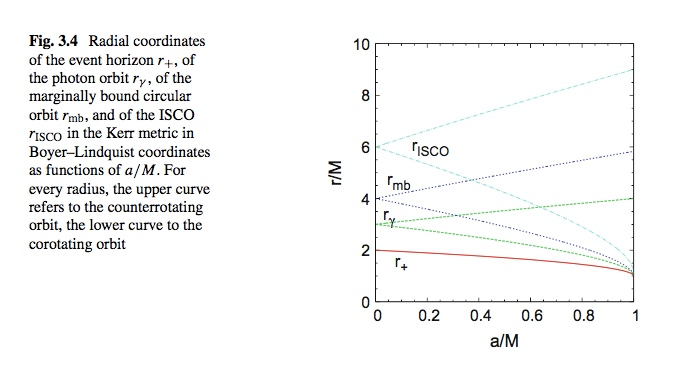
\includegraphics[scale=0.4] {figures/kerrradii.jpeg}
      \end{figure}
	\end{center}	
\end{frame}




\section{Geodesics in Kerr Spacetime}    
\begin{darkframes}

\subsection{Hamilton-Jacobi Formulation}
\begin{frame}
\Huge
Hamilton-Jacobi Formulation
\end{frame}

\begin{frame}{Hamilton-Jacobi Formulation}
    \[ \mathcal{L} = \frac{1}{2}  g_{\mu\nu} \dot{x}^\mu \dot{x}^\nu \]
    \pause
    \[ p_\mu = \frac{\partial \mathcal{L}}{\partial \dot{x}^\mu} =  g_{\mu\nu} \dot{x}^\nu \]
    \pause
    \[ \mathcal{H} = \frac{1}{2}  g^{\mu\nu} p_\mu p_\nu \]
\end{frame}

\begin{frame}{Hamilton-Jacobi Formulation}
    Hamilton's principal function
    \[ S = S \left( x^\mu ; \lambda \right)\]
    \pause
    \[ p_\mu = \frac{\partial S}{\partial x^\mu} \]
    \pause
    Hamilton-Jacobi Equation
    \pause
    \[  \frac{1}{2}  g^{\mu\nu} \frac{\partial S}{\partial x^\mu} \frac{\partial S}{\partial x^\nu} - \frac{\partial S}{\partial \lambda} =0 \]
\end{frame}

\begin{frame}{Kerr's Solution}
    	Boyer-Lindquist coordinates: $\left(t,r,\theta,\varphi\right)$
     	\begin{align*}
            ds^{2} &= -\frac{\Delta-a^{2}\sin^{2}\theta}{\varrho}dt^{2}-\left(\frac{r^{2}+a^{2}-\Delta}{\varrho}\right)2a\sin^{2}\theta dtd\varphi\nonumber \\
             & +\frac{\varrho}{\Delta}dr^{2}+\varrho d\theta^{2}+\left(\frac{\left(r^{2}+a^{2}\right)^{2}-\Delta a^{2}\sin^{2}\theta}{\varrho}\right)\sin^{2}\theta d\varphi^{2}.
      	\end{align*}
     	\pause
   	$$\varrho  = r^{2}+a^{2}\cos^{2}\theta$$
    $$\Delta =  r^{2}-2Mr+a^{2}$$
\end{frame}

\begin{frame}{Kerr's Solution}
     	\begin{align*}
            \left( \frac{\partial}{\partial s} \right)^{2} = &- \frac{A}{\varrho \Delta} \left( \frac{\partial}{\partial t} \right)^{2} - \frac{4aMr}{\varrho \Delta} \left( \frac{\partial}{\partial t} \right) \left( \frac{\partial}{\partial \varphi} \right) +\frac{\Delta}{\varrho}\left( \frac{\partial}{\partial r} \right)^2 \nonumber \\
             & + \frac{1}{\varrho} \left( \frac{\partial}{\partial \theta} \right)^{2} + \frac{\Delta - a^2 \sin^2 \theta}{\varrho \Delta \sin^{2}\theta} \left( \frac{\partial}{\partial \varphi} \right)^{2}
      	\end{align*}
    \pause
    $$A = (r^2 + a^2)^2 -a^2 \Delta \sin^2 \theta$$ 	
   	$$\varrho  = r^{2}+a^{2}\cos^{2}\theta$$
    $$\Delta =  r^{2}-2Mr+a^{2}$$
\end{frame}

\begin{frame}{Hamilton-Jacobi Formulation}
    Hamilton-Jacobi Equation
     \[ 2 \frac{\partial S}{\partial \lambda}  = g^{\mu\nu} \frac{\partial S}{\partial x^\mu} \frac{\partial S}{\partial x^\nu} \]
    \pause
    \begin{align*}
           2 \frac{\partial S}{\partial \lambda} = &- \frac{A}{\varrho \Delta} \left( \frac{\partial S}{\partial t} \right)^2 - \frac{4aMr}{\varrho \Delta} \left( \frac{\partial S}{\partial t} \right) \left( \frac{\partial S}{\partial \varphi} \right) +\frac{\Delta}{\varrho}\left( \frac{\partial S}{\partial r} \right)^2 \nonumber \\
             & + \frac{1}{\varrho} \left( \frac{\partial S}{\partial \theta} \right)^{2} + \frac{\Delta - a^2 \sin^2 \theta}{\varrho \Delta \sin^{2}\theta} \left( \frac{\partial S}{\partial \varphi} \right)^{2}
    \end{align*}   
\end{frame}

\begin{frame}{Hamilton-Jacobi Formulation}
    Hamilton Principal Function
    \[S = \frac{1}{2} \lambda \delta -\varepsilon t +\ell_z \varphi + S_r (\theta) + S_\theta (\theta)\]
	Separation of the Hamilton-Jacobi Equation. Carter Constant
	\begin{align*}
	&\Delta \left( \frac{dS_r}{dr}\right)^2 - \frac{1}{\Delta} \left[ (r^2 +a^2) \varepsilon - a \ell_z \right]^2 + (\ell_z - a \varepsilon)^2 + \delta r^2  =\\
	& -\left( \frac{dS_\theta}{d\theta}\right)^2 - \left(\frac{\ell_z^2}{\sin^2 \theta} - a^2 \varepsilon^2 + \delta a^2 \right)\cos^2 \theta = \mathcal{C}
	\end{align*}      
\end{frame}

\begin{frame}{Hamilton-Jacobi Formulation}
	Separation of the Hamilton-Jacobi Equation. Carter Constant
	\begin{align*}
	\Delta \left( \frac{dS_r}{dr}\right)^2 &= \frac{1}{\Delta} \left[ (r^2 +a^2) \varepsilon - a \ell_z \right]^2 - \left[ \mathcal{C} + (\ell_z - a \varepsilon)^2 + \delta r^2 \right]\\ 
	\left( \frac{dS_\theta}{d\theta}\right)^2 &= \mathcal{C} - \left( \frac{\ell_z^2}{\sin^2 \theta} - a^2 \varepsilon^2 + \delta a^2 \right) \cos^2 \theta	
	\end{align*}      
\end{frame}

\begin{frame}{Hamilton-Jacobi Formulation}
	\begin{align*}
	S_r &= \int \frac{\sqrt{R(r')}}{\Delta}dr'\\
	S_\theta &= \int \sqrt{\Theta(\theta')}d\theta'
	\end{align*}
	\pause 
	\begin{align*}
	R(r) &= \left[ (r^2 +a^2) \varepsilon - a \ell_z \right]^2 - \Delta \left[\mathcal{C} + (\ell_z - a \varepsilon)^2 + \delta r^2 \right]\\
	\Theta(\theta) &= \mathcal{C} - \left[ \frac{\ell_z^2}{\sin^2 \theta} + a^2 \left(\delta - \varepsilon^2 \right) \right] \cos^2 \theta
	\end{align*}      
\end{frame}

\begin{frame}{Carter Constant}
	\[\left( \frac{dS_\theta}{d\theta}\right)^2 = \mathcal{C} - \left( \frac{\ell_z^2}{\sin^2 \theta} - a^2 \varepsilon^2 + \delta a^2 \right) \cos^2 \theta\] 
	\bigskip
	\pause
	
	\[ \mathcal{C} = p_\theta^2 + p_\varphi^2 \cot^2 \theta + a^2 (\delta - \varepsilon^2) \cos^2 \theta \]     
\end{frame}

\begin{frame}{Carter Constant}
	Schwarzschild:		
	\[ \mathcal{C} = \left( p_\theta^2 + \frac{p_\varphi^2}{\sin^2 \theta} \right) - p_\varphi^2 = \ell^2 - \ell_z^2 \]   
	where $\ell = p_\theta^2 + \frac{p_\varphi^2}{\sin^2 \theta}$ is the total angular momentum.
\end{frame}

\begin{frame}{Carter Constant}
	Kerr:
	\pause		
	\begin{itemize}
	\item $\mathcal{C}$ has not a direct physical interpretation.
	\item $\mathcal{C}=0$ implies that the motion is in the equatorial plane.
	\end{itemize}
\end{frame}



\subsection{Equations of Motion}
\begin{frame}
	\huge
    {Equations of Motion}
\end{frame}

\begin{frame}{Equations of Motion}
    Hamilton Canonical Equations
    \pause
    \[ \dot{x}^\mu = p^\mu = g^{\mu \nu} p_\nu = g^{\mu\nu} \frac{\partial S}{ x^\nu} \]
\end{frame}

\begin{frame}{Equations of Motion}
    \footnotesize

    \begin{align*}
    \varrho^2 \dot{r}^2 &= R \\
    \varrho^2 \dot{\theta}^2 &= \Theta \\
    \varrho \dot{\varphi} &= \frac{1}{\Delta} \left[ 2aMr\varepsilon + (\varrho - 2Mr)\frac{\ell_z}{\sin^2 \theta} \right] \\
    \varrho \dot{t} &= \frac{1}{\Delta} \left[ A\varepsilon + 2aMr \ell_z \right]
    \end{align*}
    \pause
    \begin{align*}
    R(r) &= \left[ (r^2 +a^2) \varepsilon - a \ell_z \right]^2 - \Delta \left[\mathcal{C} + (\ell_z - a \varepsilon)^2 + \delta r^2 \right]\\
	\Theta(\theta) &= \mathcal{C} - \left[ \frac{\ell_z^2}{\sin^2 \theta} + a^2 \left(\delta - \varepsilon^2 \right) \right] \cos^2 \theta\\
    A &= (r^2 + a^2)^2 - a^2 \Delta \sin^2 \theta \\
    \varrho  &= r^{2}+a^{2}\cos^{2}\theta \\
    \Delta &= r^{2}-2Mr+a^{2} 
    \end{align*}
\end{frame}






\end{darkframes}
\begin{frame}{Gravitational Collapse of a Homogeneous Cloud of Dust}
\framesubtitle{Eddington-Finkelstein Diagram}
	\begin{center}
      \begin{figure}
      	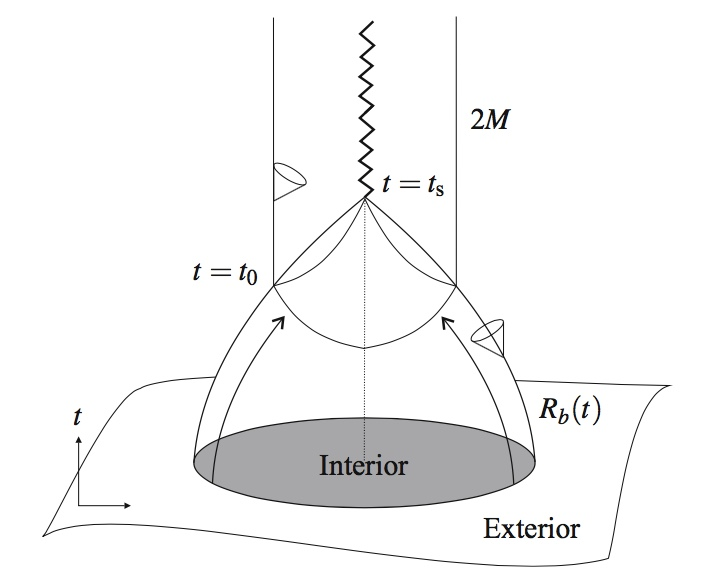
\includegraphics[scale=0.25] {figures/EFCollapse.jpeg}
      \end{figure}
	\end{center}	
\end{frame}

\begin{frame}{Gravitational Collapse of a Homogeneous Cloud of Dust}
\framesubtitle{Eddington-Finkelstein Diagram}
	\begin{center}
      \begin{figure}
      	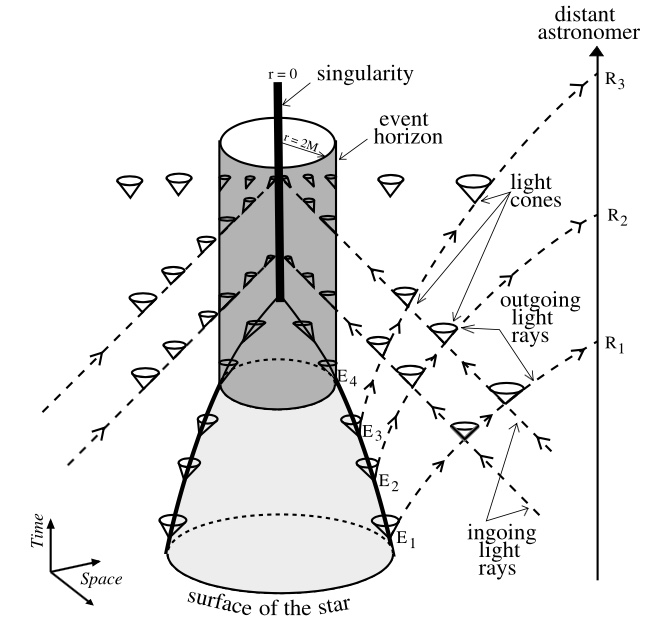
\includegraphics[scale=0.25] {figures/EFCollapse2.jpeg}
      \end{figure}
	\end{center}	
\end{frame}

\begin{darkframes}

\subsection{Inhomogeneous Dust Collapse}
\begin{frame}
	\huge
    Inhomogeneous Dust Collapse
\end{frame}

\begin{frame}{Inhomogeneous Dust Collapse}
    $\rho$ depends on both $t$ and $r$, and thus\\
    \bigskip
    \pause
    $\rho = \rho(t,r)$\\
    $m = m(r)$\\
    $b = b(r)$\\
    $a = a(t,r)$
\end{frame}



  		\begin{frame}{Next Lecture}
        	\Large
			{06. Black Holes Astrophysics}
		\end{frame}
  
  \end{darkframes}
\end{document}
